\TFRGB{Utilisation du module  \og pgffor \fg  chargé automatiquement avec TikZ }{Package used :  \og pgffor \fg (automatically loaded with TikZ) }


%\subsection{Répétition à 1 variable}
\SbSSCT{Répétition à 1 variable}{One variable repetition}

%\psLoop{5}{ \DFR }
\begin{tabular}{|c|} \hline  

\tikz \foreach \x in {1,...,10} \fill[blue](\x,0) circle (0.4cm);
\\  \hline  
\BS{tikz} \BSS{foreach} \BSR{x} in \AC{1,...,10} \BS{fill}[blue](\BSR{x},0) circle (0.4cm);
\\ \hline 
Variable \BSR{x} : position en X 
\\ \hline 
\end{tabular} 

%\subsection{Répétition à 2 variables}
\SbSSCT{Répétition à 2 variables}{Two variables repetition}

\begin{tabular}{|c|} \hline  
\TFRGB{Liste de variables numériques}{Numerical variables}
\\ \hline 
\tikz \foreach \pos/\y in {1/10,2/20,3/30,4/40,5/50,6/60,7/70,8/80,9/90,10/100} \fill[color=blue!\y](\pos,0) circle (0.5cm);
\\ \hline  
\BS{tikz} \BS{foreach} \BSR{pos}/\BSB{y} in \AC{1/10,2/20,3/30,4/40,5/50,6/60,7/70,8/80,9/90,10/100} \\ \BS{fill}[color=blue!\BSB{y}](\BSR{pos},0) circle (0.5cm);
\\ \hline 
Variable \BSR{pos} : position en X \hspace{1cm} Variable \BSB{y} : couleur
\\ \hline 
\end{tabular} 

\bigskip

\begin{tabular}{|c|} \hline
\TFRGB{Liste de variables mixtes}{Composite variables}
\\ \hline   
\tikz \foreach \x/\col in {1/red,3/green,5/magenta,7/blue}  \shade[ball color=\col](\x,0) circle (1);
\\ \hline  
\BS{tikz} \BS{foreach} \BSR{x}/\BSB{col} in {1/red,3/green,5/magenta,7/blue}  \BS{shade}[ball color=\BSB{col}](\BSR{x},0) circle (1);
\\  \hline 
Variable \BSR{x} : position en X  \hspace{1cm}  Variable \BSB{col} : couleur 
\\ \hline 
\end{tabular} 



\bigskip

\begin{tabular}{|c|} \hline
\TFRGB{Liste de variables avec un pas}{Variables with a step}
\\ \hline   
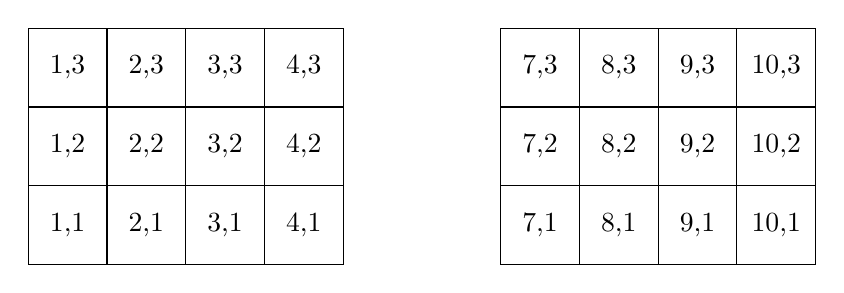
\begin{tikzpicture}
  \foreach \x in {1,2,...,4,7,8,...,10}
    \foreach \y in {1,...,3}
    {      \draw (\x,\y) +(-.5,-.5) rectangle ++(.5,.5);
      \draw (\x,\y) node{\x,\y};
    }
\end{tikzpicture}
\\ \hline  
\parbox{12cm}{ 
\BS{begin}\AC{tikzpicture}\\
\BS{foreach} \BSR{x} in\AC{1,2,...,4,7,8,...,10} \\
\BS{foreach} \BSB{y} in \AC{1,...,3} \\
\AC{  \BS{draw} (\BSR{x},\BSB{y}) +(-.5,-.5) rectangle ++(.5,.5);
\BS{draw} (\BSR{x},\BSB{y}) node{\BSR{x},\BSB{y}}; }\\
\BS{end}\AC{tikzpicture} \\
}
\\ \hline 
Variable \BSR{x} : position en X  \hspace{1cm}  Variable \BSR{y} : position en Y 
\\ \hline 

\end{tabular}

\bigskip
\begin{tabular}{|l|l|} \hline 
 \multicolumn{2}{|c|}{ \TFRGB{Exemples de liste}{List example }}
 \\ \hline 
\foreach \x in {1,...,6} {\x, }
&  
\BS{foreach} \BSR{x} in \AC{1,...,6} \AC{\BSR{x}, }
\\ \hline 
\foreach \x in {1,3,...,11} {\x, }
&  
\BS{foreach} \BSR{x} in \AC{1,3,...,11} \AC{\BSR{x}, }
\\ \hline 
\foreach \x in {Z,X,...,M} {\x, }
&  
\BS{foreach} \BSR{x} in \AC{Z,X,...,M} \AC{\BSR{x}, }
\\ \hline 
\foreach \x in {2^1,2^...,2^7} {$\x$, }
&  
\BS{foreach} \BSR{x} in \AC{2\^{}1,2\^{}...,2\^{}7} \AC{\BSR{x}, }
\\ \hline
\foreach \x in {0cm,0.5cm,...cm,3cm} {$\x$, }
&  
\BS{foreach} \BSR{x} in \AC{0cm,0.5cm,...cm,3cm} \AC{\BSR{x}, }
\\ \hline
\foreach \x in {A_1,..._1,H_1} {$\x$, } 
&  
\BS{foreach} \BSR{x} in \AC{A\_1,...\_1,H\_1} \AC{\BSR{x}, }
\\ \hline
\end{tabular} 




\bigskip
\begin{tabular}{|c|} \hline 
\TFRGB{Variables numériques avec opération}{Calculation on variables}
\\ \hline  

\begin{tikzpicture}
   \foreach \x in {0,20,...,360}{ \filldraw[red] (0,0) .. controls (\x+10:1) .. (\x:3) .. controls (\x-10:1) .. (0,0);}
    \foreach \x in {10,30,...,370}{ \filldraw[blue] (0,0) .. controls (\x+10:1) .. (\x:3) .. controls (\x-10:1) .. (0,0);}  
\end{tikzpicture}
\\ \hline  
\parbox{12cm}{ 
\BS{begin}\AC{tikzpicture}\\
   \BS{foreach} \BSR{x} in {0,20,...,360}\AC{ \BS{filldraw}[red] (0,0) .. controls (\BSR{x}+10:1) .. (\BSR{x}:1) .. controls (\BSR{x}-10:1) .. (0,0);} \\
    \BS{foreach}  \BSR{x} in {10,30,...,370}\AC{ \BS{filldraw}[blue] (0,0) .. controls (\BSR{x}+10:3) .. (\BSR{x}:3) .. controls (\BSR{x}-10:3) .. (0,0);}  \\
\BS{end}\AC{tikzpicture} \\

}
\\ \hline 
Variable \BSR{x} : angle 
\\ \hline 
\end{tabular} 




%\subsection{Répétition à 2 variables - boucles imbriquées}
\SbSSCT{Répétition à 2 variables - boucles imbriquées}{Nested loops}

\begin{tabular}{|c|c|} \hline  
 \multicolumn{2}{|c|}{\TFRGB{Ordre des boucles imbriquées}{Order of the nested loops }}
\\ \hline 

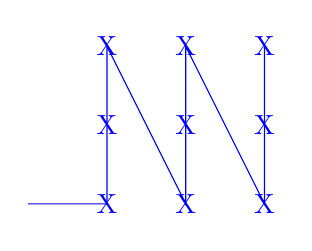
\begin{tikzpicture}[blue]
\draw (0,0)
\foreach \x in {1,2,3}
{\foreach \y in {0,1,2}
{-- (\x,\y) node{X}}};
\end{tikzpicture}
&  
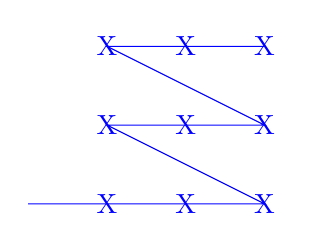
\begin{tikzpicture}[blue]
\draw (0,0)
\foreach \y in {0,1,2}
\foreach \x in {1,2,3}
{-- (\x,\y) node{X}};
\end{tikzpicture}
\\ \hline 
\parbox{5cm}{ 
\BS{begin}\AC{tikzpicture} \\
\BS{draw} (0,0) \\
\BS{foreach} \BSR{x} in \AC{1,2,3} \\
\BS{foreach} \BSB{y} in \AC{0,1,2} \\
\AC{-- (\BSR{x},\BSB{y}) node\AC{X}};\\
\BS{end}\AC{tikzpicture} \\ } 
&  
\parbox{5cm}{ 
\BS{begin}\AC{tikzpicture} \\
\BS{draw} (0,0) \\
\BS{foreach} \BSB{y} in \AC{0,1,2}\\
\BS{foreach} \BSR{x} in   \AC{1,2,3}\\
\AC{-- (\BSR{x},\BSB{y}) node\AC{X}};\\
\BS{end}\AC{tikzpicture} \\ } 
\\ \hline 
\end{tabular} 




